\documentclass[tikz,border=2mm]{standalone}

\begin{document}
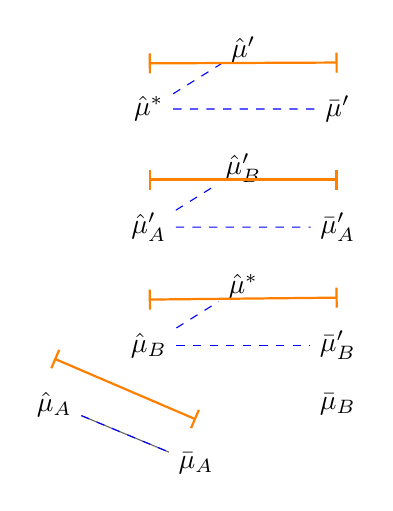
\begin{tikzpicture}[scale=3]
    \node (a) at (0,0) {$\hat{\mu}_A$};
    \node (b) at (0.6,-0.25) {$\bar{\mu}_A$};
    \draw [black!60] (a) -- (b);
    \draw[|-|,orange,thick] ([shift={(0,0.1)}]a.north)--([shift={(0,0.1)}]b.north);
    \draw[dashed,blue] (a)--(b);
    
    \node (c) at (0.4,0.25) {$\hat{\mu}_B$};
    \node (d) at (0.8,0.5) {$\hat{\mu}^*$};
    \node (e) at (1.2,0.25) {$\bar{\mu}'_B$};
    \node (f) at (1.2,0) {$\bar{\mu}_B$};
    
    \draw[dashed,blue] (c)--(d);
    \draw[|-|,orange,thick] ([shift={(0,0.1)}]c.north)--([shift={(0,0.1)}]e.north);
    \draw[dashed,blue] (c)--(e);
    
    \node (g) at (0.4,0.75) {$\hat{\mu}'_A$};
    \node (h) at (0.8,1) {$\hat{\mu}'_B$};
    \node (i) at (1.2,0.75) {$\bar{\mu}'_A$};
    
    \draw[dashed,blue] (g)--(h);
    \draw[|-|,orange,thick] ([shift={(0,0.1)}]g.north)--([shift={(0,0.1)}]i.north);
    \draw[dashed,blue] (g)--(i);
    
    \node (j) at (0.4,1.25) {$\hat{\mu}^{*}$};
    \node (k) at (0.8,1.5) {$\hat{\mu}'$};
    \node (l) at (1.2,1.25) {$\bar{\mu}'$};
    
    \draw[dashed,blue] (j)--(k);
    \draw[|-|,orange,thick] ([shift={(0,0.1)}]j.north)--([shift={(0,0.1)}]l.north);
    \draw[dashed,blue] (j)--(l);
\end{tikzpicture}
\end{document}